\documentclass[10pt,aspectratio=169]{beamer}

% ---------- Пакеты ----------
% pdfLaTeX — как в примере; LuaLaTeX также поддерживается.
\usepackage{iftex}
\ifPDFTeX
  \usepackage[utf8]{inputenc}
  \usepackage[T2A]{fontenc}
\else
  \usepackage{fontspec}
  \setsansfont{DejaVu Sans}
  \setmainfont{DejaVu Sans}
  \setmonofont{DejaVu Sans Mono}
\fi
\usepackage[russian]{babel}
\usepackage{amsmath,amssymb}
\usepackage{graphicx}
\usepackage{booktabs}
\usepackage{xcolor}
\usepackage{pgfpages}

% ---------- Тема: как в примере ----------
\usetheme{Madrid}
\usecolortheme{seahorse}
\setbeamertemplate{navigation symbols}{}
\setbeamertemplate{footline}[frame number]
\definecolor{myblue}{RGB}{76,154,255}
\definecolor{myorange}{RGB}{255,171,76}
\definecolor{mygreen}{RGB}{142,209,142}
\setbeamercolor{block title}{fg=black,bg=myblue!25}
\setbeamercolor{block body}{fg=black,bg=myblue!7}

% ---------- Сценарий выступления ----------
% Обычная версия скрывает заметки.
% PDF с заметками справа: см. команду в README.md.
\ifdefined\shownotes
  \setbeameroption{show notes on second screen=right}
\else
  \setbeameroption{hide notes}
\fi

% ---------- Метаданные ----------
\title[Анализ графа модели]{Критерии выбора элементов\\графа математической модели}
\subtitle{Лабораторная работа №2. Вариант 7--1--4}
\author{ФИО: \underline{\hspace{4cm}}}
\institute{Группа: \underline{\hspace{2.5cm}}}
\date{}

\begin{document}

% ================== Слайд 1 ==================
\begin{frame}
\titlepage
\note{Около 25 секунд. Цель работы — разработать критерий выбора структурных элементов математической модели из первой лабораторной. Рассматривается модель тележки на пружине. В соответствии с вариантом 7–1–4 распределения параметров оцениваются методом SMC, вмешательство выполняется занулением наблюдаемого входа, а различия распределений измеряются статистикой Колмогорова — Смирнова.\par\medskip Что показать: Назвать цель и выбранную тройку методов.}
\end{frame}

% ================== Слайд 2 ==================
\begin{frame}{Математическая модель и структурные элементы}

\[
 a=-kx-cv+b,\qquad k=\omega^2,\quad c=2\zeta\omega,\quad x'=v.
\]
\begin{center}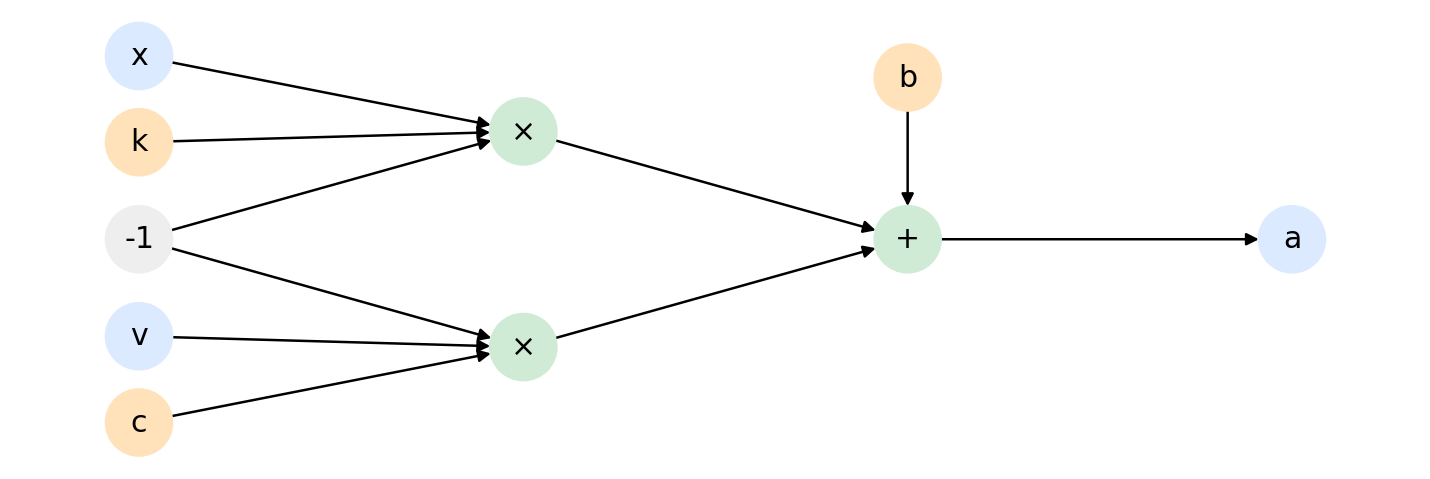
\includegraphics[width=.96\textwidth,height=.35\textheight,keepaspectratio]{figures/model_graph.png}\end{center}
\begin{itemize}
\item $x\to a$: ветвь упругой силы $-kx$; $v\to a$: ветвь сопротивления $-cv$.
\item $b$ --- служебный параметр смещения измерений.
\end{itemize}
\footnotesize Удаление ветви правой части не означает удаления переменной состояния.

\note{Около 40 секунд. Модель описывает ускорение как сумму действия пружины, сопротивления и смещения измерений. Коэффициент k равен жёсткости, делённой на массу; коэффициент c — сопротивлению, делённому на массу. На графе выделяются ветви минус k на x и минус c на v. Именно для них принимается решение о сохранении. Удаление ветви означает исключение соответствующего слагаемого с повторной оценкой остальных коэффициентов. Координата и скорость как переменные состояния при этом сохраняются.\par\medskip Что показать: Показать путь от x к произведению и от v к произведению, затем к сумме.}
\end{frame}

% ================== Слайд 3 ==================
\begin{frame}{Данные и протокол вычислительного эксперимента}

\small
\begin{tabular}{lcc}\toprule Набор & $c$ & Число точек\\\midrule
Синтетика с сопротивлением & $0{,}18$ & 600\\
Контроль без сопротивления & $0$ & 600\\
Тележка, Science (2009) & неизвестен & 870\\\bottomrule\end{tabular}
\begin{center}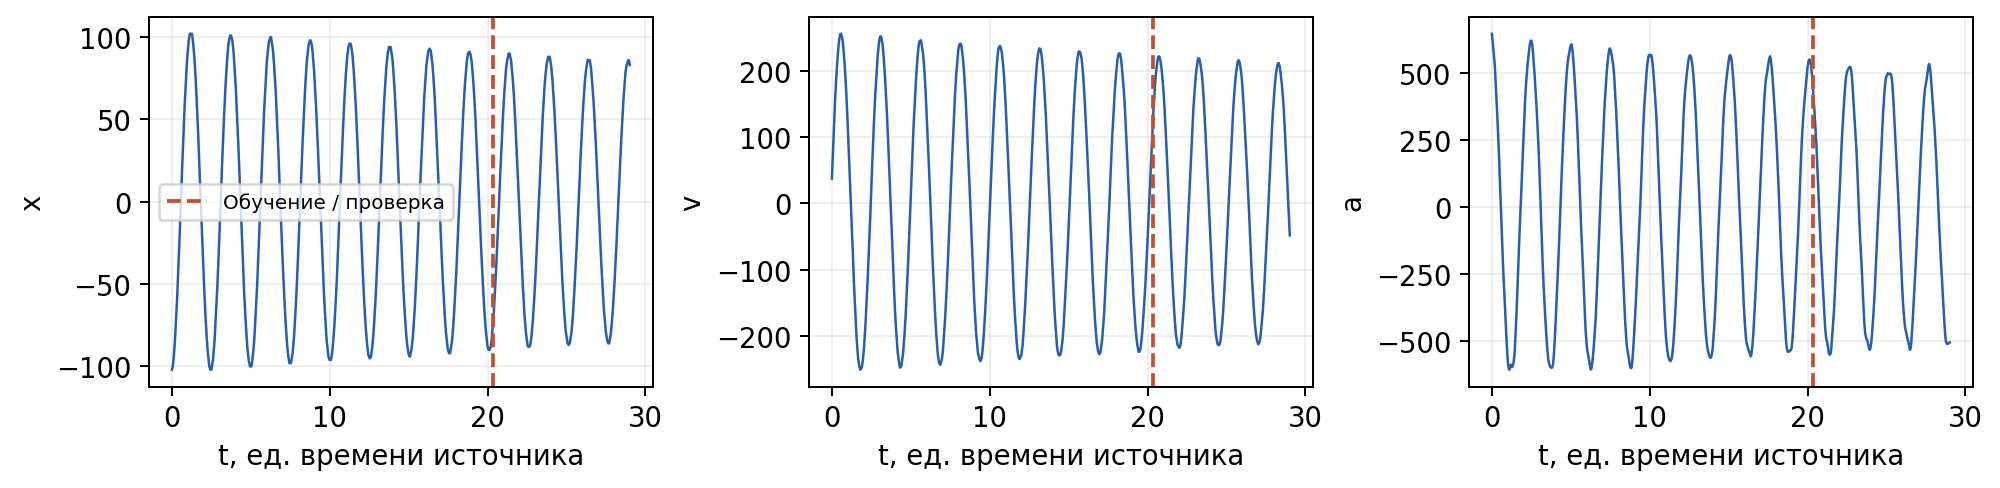
\includegraphics[width=.96\textwidth,height=.35\textheight,keepaspectratio]{figures/real_data.png}\end{center}
\footnotesize На графиках --- реальные данные. Первые 70\% ряда: обучение; последние 30\%: проверка.
Синтетика: шум ускорения $\sigma=0{,}08$, $k=6{,}25$, $b=0$.

\note{Около 40 секунд. Используются три набора: синтетическая система с сопротивлением, контроль с нулевым сопротивлением и реальные данные тележки. В синтетике правильная структура известна заранее. На графике показаны реальные координата, скорость и ускорение. Вертикальная линия отделяет обучающую часть от проверочной. Разбиение выполняется по времени, чтобы поздние наблюдения не участвовали в оценке. В синтетике шум добавлен к ускорению, а координата и скорость считаются известными без ошибок. Для реальных данных использованы производные авторов.\par\medskip Что показать: Показать границу 70/30 и объяснить роль контрольного опыта.}
\end{frame}

% ================== Слайд 4 ==================
\begin{frame}{Оценка распределений параметров методом SMC}

\[
 \theta=(k,c,b),\quad p(\theta\mid D)\propto p(\theta)L(D\mid\theta),
 \qquad \pi_\beta\propto p(\theta)L^\beta,\quad \beta:0\to1.
\]
\begin{enumerate}
\item Инициализация $N=2048$ частиц из нормального prior.
\item Перевзвешивание; адаптивный шаг температуры: $ESS\ge0{,}8N$.
\item Систематический ресемплинг и перемешивание; повтор до $\beta=1$.
\end{enumerate}
\[
 \ell_{\mathrm{MSE}}=-\frac{\sum r_i^2}{2\sigma^2},\qquad
 \ell_{\mathrm{MAE}}=-\frac{\sqrt2\sum|r_i|}{\sigma}.
\]
\footnotesize Частица --- один набор $(k,c,b)$. Prior и масштаб шума фиксируются по исходному train.

\note{Около 55 секунд. SMC оценивает распределение, а не одну оптимальную точку. Каждая частица — один набор коэффициентов k, c и b. Сначала частицы выбираются из распределения до учёта данных, затем последовательно переходят к апостериорному распределению через увеличение температуры бета от нуля до единицы. На каждом этапе выполняются перевзвешивание, ресемплинг и перемешивание. Шаг температуры выбирается по эффективному размеру выборки. Проверяются два правдоподобия: нормальное для квадратичной ошибки и Лапласа для абсолютной. При вмешательствах исходные prior и масштаб шума не меняются.\par\medskip Что показать: Показать последовательность prior \(\to\) промежуточные цели \(\to\) posterior.}
\end{frame}

% ================== Слайд 5 ==================
\begin{frame}{Контроль численной точности SMC}

\footnotesize Для MSE и нормального prior апостериорное распределение известно аналитически.
\begin{center}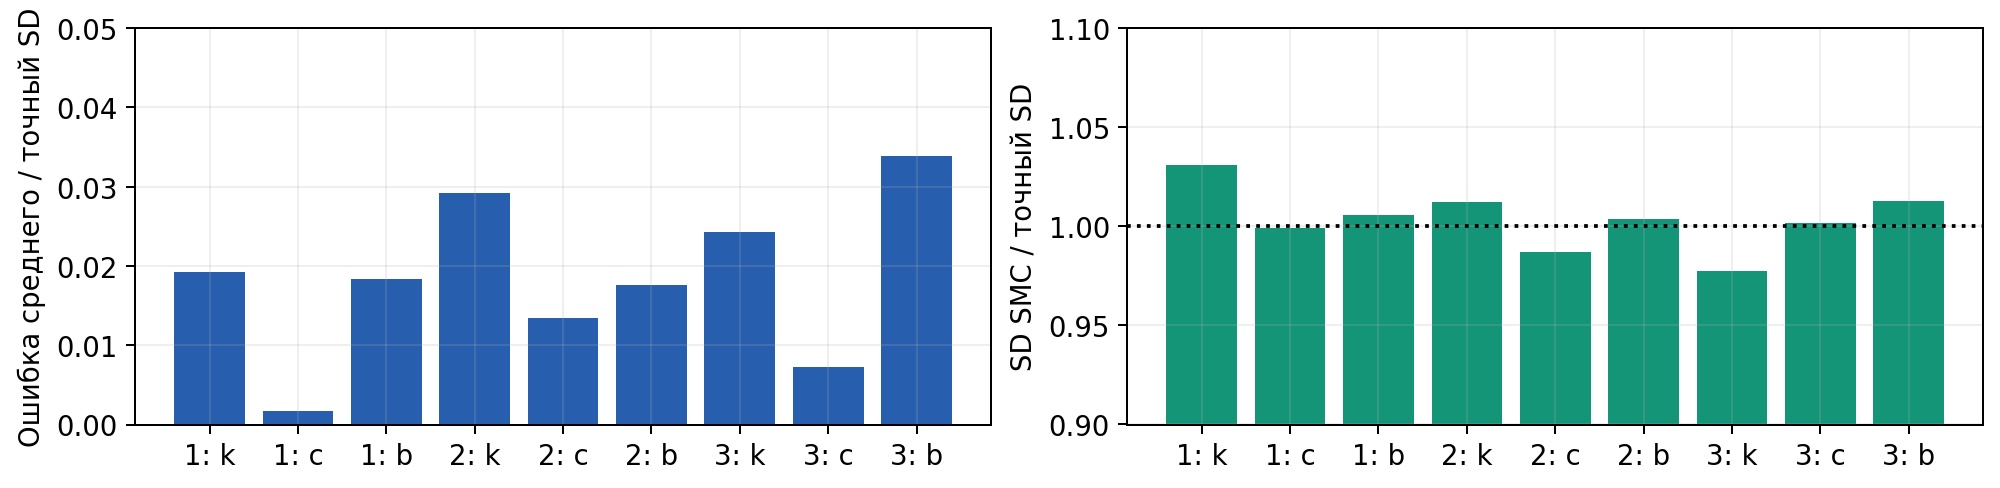
\includegraphics[width=.96\textwidth,height=.55\textheight,keepaspectratio]{figures/smc_validation.png}\end{center}
\footnotesize Группы 1, 2, 3: синтетика с трением, контроль, реальные данные.
Максимальная ошибка среднего: $0{,}034$ точного SD; отношение SD: $0{,}978$--$1{,}031$.

\note{Около 40 секунд. Для линейной модели с нормальным шумом и нормальным prior существует точное решение. Оно используется как независимый контроль SMC. Слева показана ошибка оценённого среднего в единицах точного стандартного отклонения. Справа — отношение стандартного отклонения SMC к точному. По горизонтали перечислены три коэффициента в каждом из трёх опытов. Максимальная ошибка среднего составляет примерно ноль целых тридцать четыре тысячных стандартного отклонения. Отношение дисперсионных масштабов близко к единице. Это подтверждает численную точность для данной проверяемой постановки.\par\medskip Что показать: Показать малые столбцы слева и близость столбцов справа к линии 1.}
\end{frame}

% ================== Слайд 6 ==================
\begin{frame}{Исходные распределения: синтетика с сопротивлением}
\begin{center}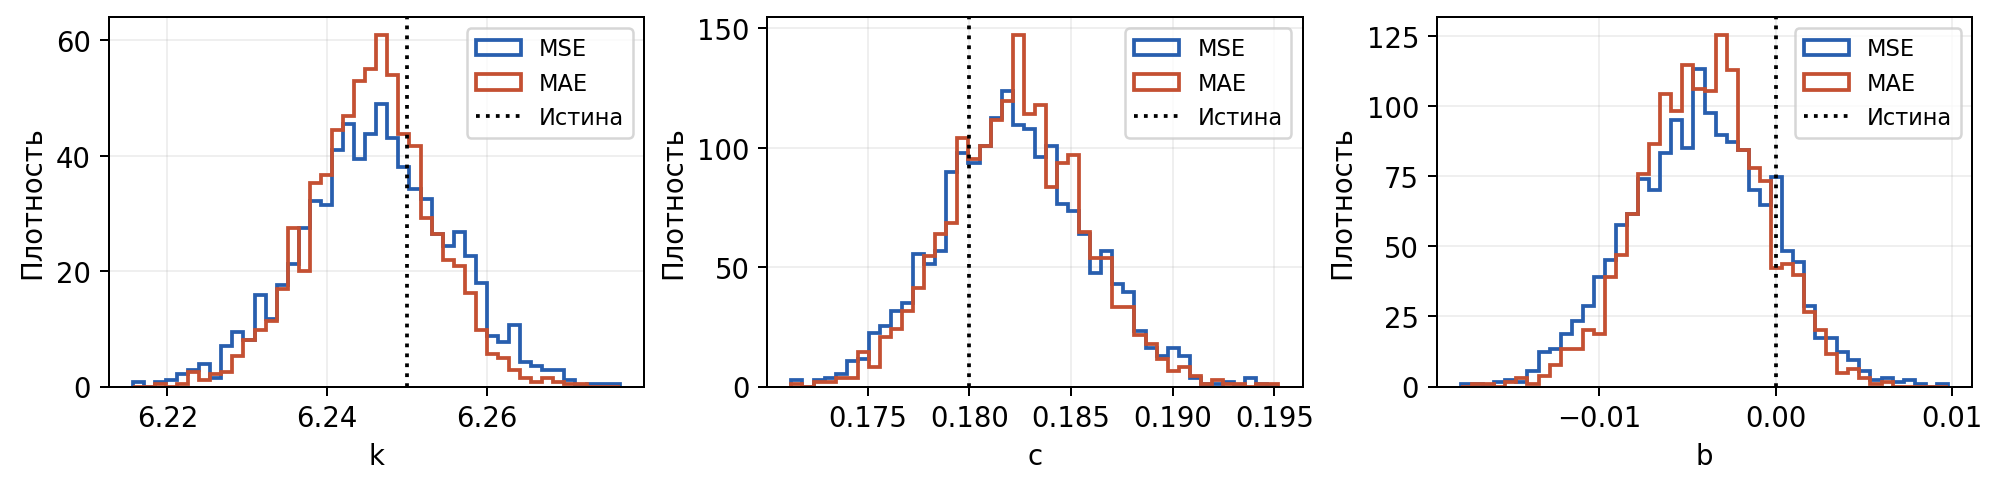
\includegraphics[width=.96\textwidth,height=.57\textheight,keepaspectratio]{figures/posterior_0.png}\end{center}
\begin{block}{Интерпретация плотности}
Ось абсцисс --- значение коэффициента; площадь под кривой на интервале --- вероятность.
Пунктир --- истинные $k=6{,}25$, $c=0{,}18$, $b=0$.
\end{block}

\note{Около 40 секунд. На графиках показаны исходные апостериорные распределения трёх коэффициентов для синтетики с сопротивлением. Синий контур соответствует MSE, оранжевый — MAE. Пунктир отмечает истинные значения. Плотность показывает концентрацию вероятных значений параметра: вероятность интервала равна площади под кривой на этом интервале. Узкие распределения указывают на небольшую неопределённость в рамках выбранной модели шума. MSE и MAE дают близкие оценки, а истинные значения находятся в основной области полученных распределений.\par\medskip Что показать: Назвать оси, цвета и истинное значение c; не называть высоту плотности вероятностью.}
\end{frame}

% ================== Слайд 7 ==================
\begin{frame}{Интервенция и расстояние между распределениями}

\[
 D^{(x)}:\ x_i\leftarrow0,\qquad D^{(v)}:\ v_i\leftarrow0,\qquad a_i\ \text{не меняется},
 \qquad D_j=\sup_z|\widehat F_j(z)-\widehat G_j(z)|.
\]
\begin{center}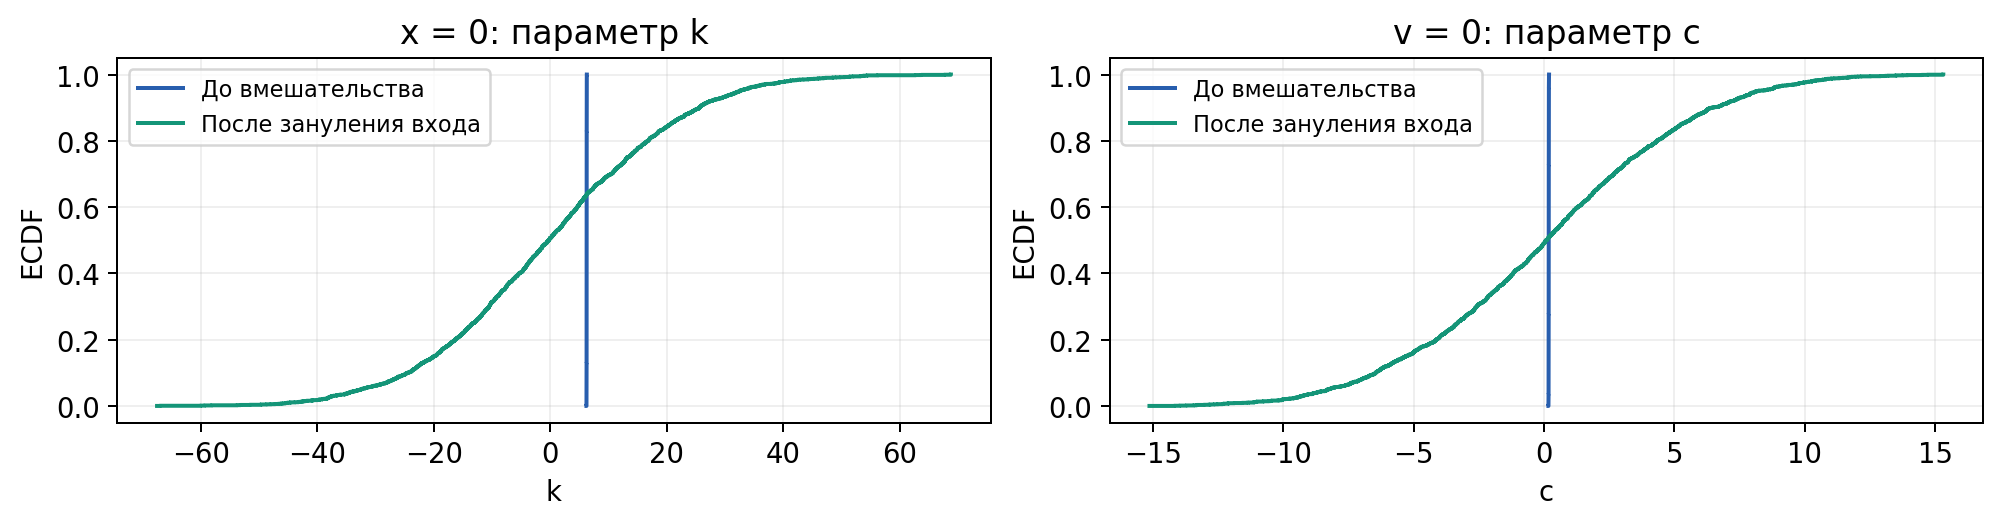
\includegraphics[width=.96\textwidth,height=.46\textheight,keepaspectratio]{figures/intervention_ecdf.png}\end{center}
\footnotesize ECDF --- доля частиц с коэффициентом $\le z$. KS --- максимальный вертикальный разрыв.
Зануление таблицы не является физическим воздействием с пересчётом ускорения.

\note{Около 50 секунд. В обучающей таблице по очереди зануляется координата или скорость, а ускорение сохраняется. После этого распределения коэффициентов оцениваются повторно. Нижние по смыслу кривые здесь — эмпирические функции распределения. Для каждого значения по горизонтали ECDF показывает долю частиц с меньшим или равным коэффициентом. KS равен максимальному вертикальному расстоянию между исходной и интервенционной кривыми. На левом графике после зануления координаты расширяется распределение k, на правом после зануления скорости расширяется распределение c. Это диагностика таблицы наблюдений, а не моделирование физической остановки.\par\medskip Что показать: Показать резкий исходный подъём ECDF и пологую кривую после зануления.}
\end{frame}

% ================== Слайд 8 ==================
\begin{frame}{Потеря идентифицируемости при занулении входа}
\begin{center}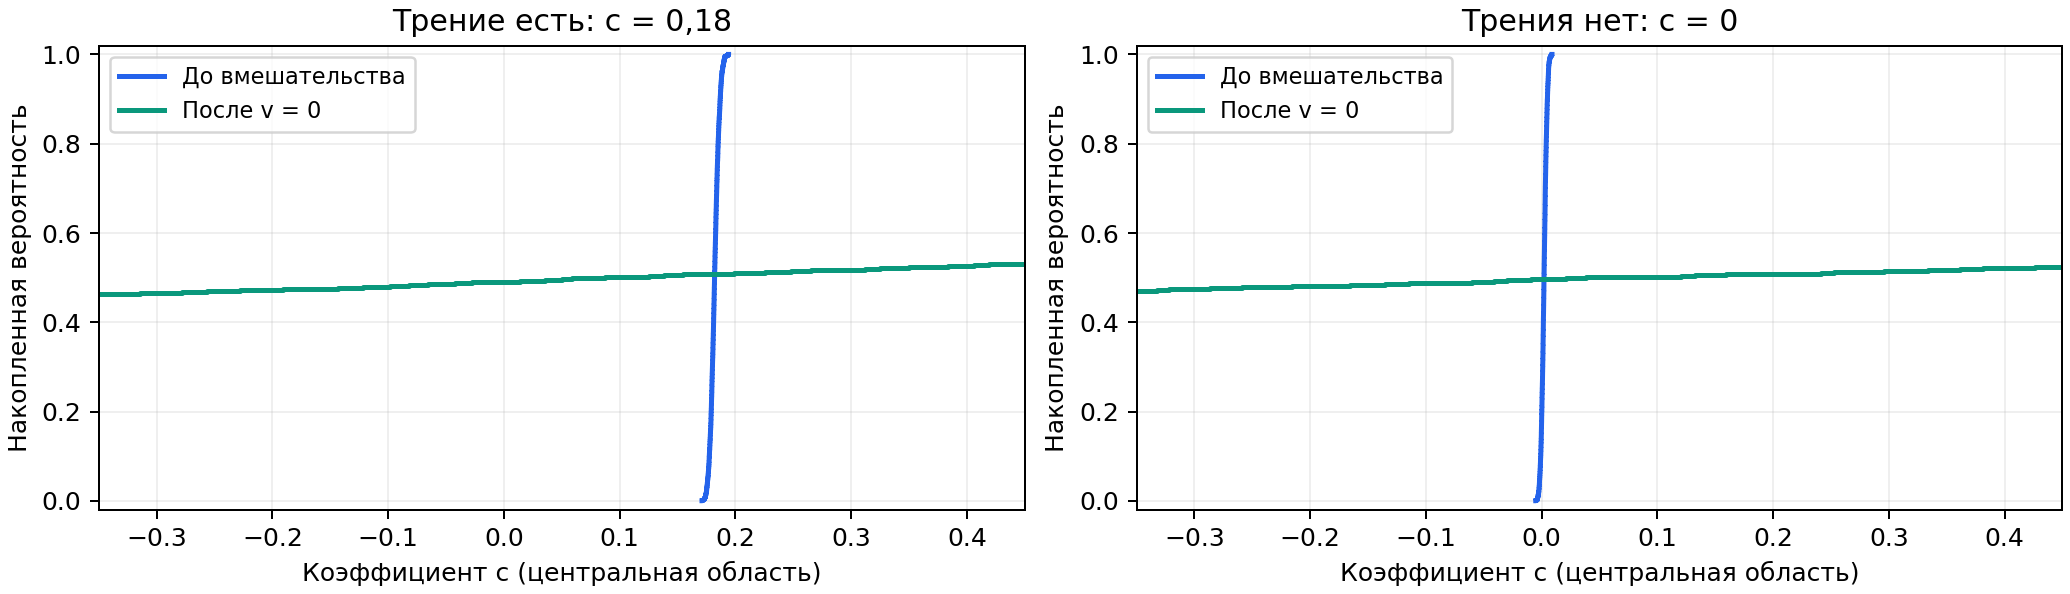
\includegraphics[width=.96\textwidth,height=.5\textheight,keepaspectratio]{figures/ks_control.png}\end{center}
\[
 v_i=0\ \forall i\ \Longrightarrow\ L\text{ не зависит от }c
 \ \Longrightarrow\ p(c\mid D^{(v)})=p(c).
\]
\footnotesize При независимом prior. $D_c\approx0{,}507$ при трении и $0{,}502$ без трения:
большое KS не является достаточным условием сохранения ветви.

\note{Около 50 секунд. Контрольный опыт демонстрирует ограничение распределительного расстояния. После зануления скорости слагаемое c на v равно нулю при любом c. Правдоподобие перестаёт зависеть от этого коэффициента, поэтому при независимом prior его апостериорное распределение возвращается к prior. Это происходит и при наличии реального сопротивления, и при его отсутствии. Поэтому KS в обоих опытах близок к половине, хотя структурные решения должны быть разными. Большой сдвиг распределения здесь свидетельствует о потере идентифицируемости, а не автоматически о необходимости ветви.\par\medskip Что показать: Сопоставить два опыта и одинаково широкие зелёные распределения.}
\end{frame}

% ================== Слайд 9 ==================
\begin{frame}{Формальный критерий удаления ветви}

\[
 s_j^{(m)}=\frac{|\theta_j^{(m)}|\operatorname{sd}(X_j)}{\operatorname{sd}(a)},
 \qquad E_j=Q_{0.95}(s_j^{(1)},\ldots,s_j^{(N)}),
 \qquad \Delta_j=\frac{\operatorname{RMSE}_{\rm reduced}}{\operatorname{RMSE}_{\rm full}}-1.
\]
\begin{block}{Правило}
Удалить ветвь, если $E_j<0{,}01$ и $\Delta_j\le0{,}05$; иначе сохранить.
При расхождении MSE и MAE --- сохранить.
\end{block}
\small
\begin{itemize}
\item $\operatorname{sd}(-c v)=|c|\operatorname{sd}(v)$: $s_j$ сравнивает масштабы ветви и ускорения.
\item Вклад оценивается на train; RMSE --- на test после переоценки остальных коэффициентов.
\item Это относительный масштаб, а не доля дисперсии; сумма вкладов не обязана равняться 1.
\end{itemize}

\note{Около 60 секунд. Для структурного решения используются два дополнительных показателя. Для каждой частицы модуль коэффициента умножается на стандартное отклонение входа и делится на стандартное отклонение ускорения. Это отношение масштабов, поскольку стандартное отклонение произведения постоянного коэффициента на переменную равно модулю коэффициента на стандартное отклонение переменной. Далее берётся девяносто пятый процентиль по частицам. Второй показатель — относительный рост RMSE после удаления ветви и повторной оценки остальных коэффициентов. Ветвь удаляется только при вкладе меньше одного процента и росте ошибки не больше пяти процентов. Пороги являются практическими допусками, а не теоретическими константами.\par\medskip Что показать: Объяснить назначение sd и 95\%-квантили, затем оба условия удаления.}
\end{frame}

% ================== Слайд 10 ==================
\begin{frame}{Структурные решения на синтетических данных}
\begin{center}\small\begin{tabular}{llrrl}\toprule Опыт & Ветвь & $E_j$ & $\Delta_j$ & Решение\\\midrule С трением & $x\to a$ & $100.45\%$ & $1460.72\%$ & сохранить \\
С трением & $v\to a$ & $7.49\%$ & $45.91\%$ & сохранить \\
Без трения & $x\to a$ & $100.12\%$ & $5985.78\%$ & сохранить \\
Без трения & $v\to a$ & $0.23\%$ & $-0.35\%$ & удалить \\
\bottomrule\end{tabular}\end{center}
\begin{itemize}
\item Ветвь пружины сохраняется в обоих опытах.
\item Сопротивление сохраняется при $c=0{,}18$ и удаляется при $c=0$.
\item Решения MSE и MAE совпадают; в таблице --- результаты MSE.
\end{itemize}

\note{Около 40 секунд. В таблице приведены решения на данных с известной структурой. Ветвь пружины сохраняется в обоих опытах. При ненулевом сопротивлении вклад скорости составляет примерно семь с половиной процентов, а удаление повышает RMSE почти на сорок шесть процентов, поэтому ветвь сохраняется. В контроле без сопротивления вклад около нуля целых двадцати трёх сотых процента, а ошибка после удаления немного уменьшается. Здесь удаление допустимо. Таким образом, критерий правильно различает эти два контрольных случая; это не доказательство универсальной корректности для любых моделей.\par\medskip Что показать: Прочитать две строки ветви скорости; пояснить, что проценты в таблице не доли от 0 до 1.}
\end{frame}

% ================== Слайд 11 ==================
\begin{frame}{Реальные данные: распределения параметров}
\begin{center}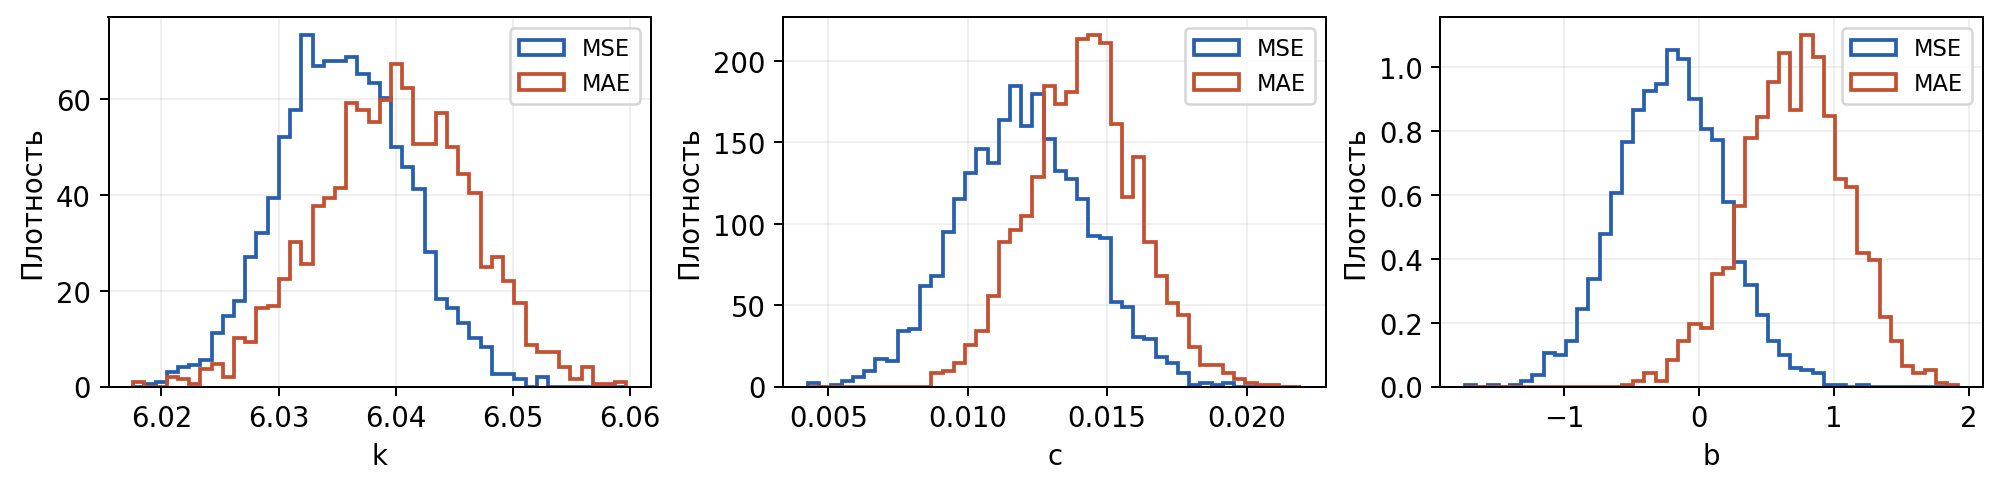
\includegraphics[width=.96\textwidth,height=.56\textheight,keepaspectratio]{figures/posterior_2.png}\end{center}
\begin{itemize}
\item Оценки $c$ положительны, однако значимость коэффициента не равна необходимости ветви.
\item Выбор функции ошибки влияет на распределения; решения об удалении проверяются для MSE и MAE.
\end{itemize}

\note{Около 40 секунд. На реальных данных неизвестен истинный набор коэффициентов. Сравнение показывает, что выбор MSE или MAE заметен в положениях и ширинах распределений. Коэффициент сопротивления оценивается положительным. Однако наличие ненулевой оценки ещё не означает, что ветвь необходима для заданной точности предсказания ускорения. Для этого отдельно оцениваются её относительный вклад и изменение ошибки на проверочной части. Интервалы условны относительно модели шума и уже выполненной авторами обработки производных.\par\medskip Что показать: Показать различие MSE и MAE и положительную оценку c.}
\end{frame}

% ================== Слайд 12 ==================
\begin{frame}{Зависимость KS от интенсивности интервенции}
\begin{center}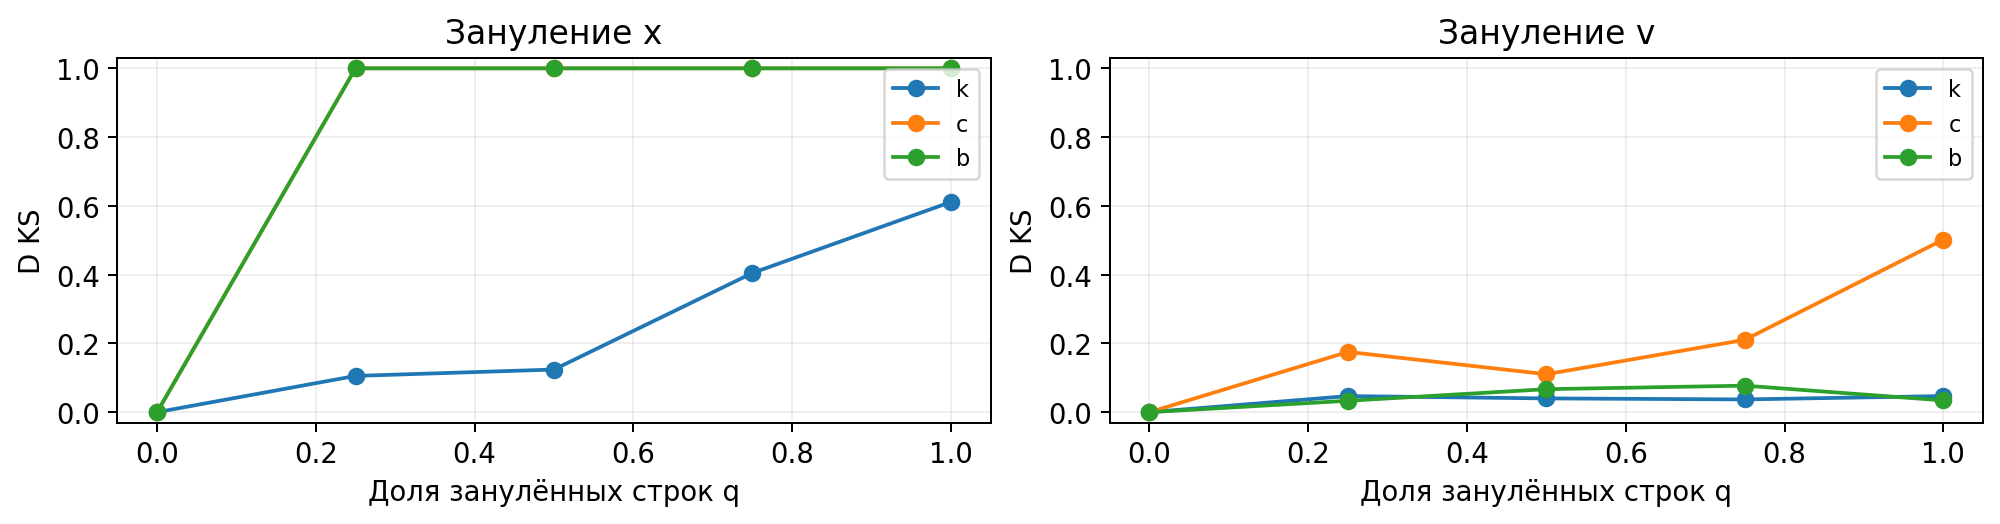
\includegraphics[width=.96\textwidth,height=.57\textheight,keepaspectratio]{figures/dose_real.png}\end{center}
\footnotesize $q$ --- доля занулённых строк; $q=1$ --- полное зануление.
Расчёт для MSE, вложенные маски, одна реализация на $q$; доверительные полосы не оценивались.

\note{Около 40 секунд. Интенсивность вмешательства задаётся долей занулённых строк q. При нуле используется исходная выборка частиц, поэтому расстояние равно нулю по определению. При единице зануляется весь выбранный вход. Показаны изменения распределений всех трёх коэффициентов для реальных данных. Зависимость не обязана быть монотонной: при частичном удалении данных остальные коэффициенты могут компенсировать нарушенную связь. Здесь для каждой интенсивности используется одна вложенная маска, поэтому график служит анализом чувствительности без оценки доверительных полос.\par\medskip Что показать: Назвать оси, левую и правую панели; показать, что меняются и другие коэффициенты.}
\end{frame}

% ================== Слайд 13 ==================
\begin{frame}{Структурные решения на реальных данных}
\begin{center}\small\begin{tabular}{llrrl}\toprule Опыт & Ветвь & $E_j$ & $\Delta_j$ & Решение\\\midrule Тележка & $x\to a$ & $100.13\%$ & $3488.35\%$ & сохранить \\
Тележка & $v\to a$ & $0.64\%$ & $1.13\%$ & удалить \\
\bottomrule\end{tabular}\end{center}
\begin{block}{Результат при заданных допусках}
Ветвь пружины сохраняется. Удаление сопротивления увеличивает RMSE
на $1{,}13\%$ при вкладе $0{,}64\%$ и допускается для ускорения.
\end{block}
\small Совпадение решений MSE и MAE не доказывает отсутствие физического трения.
Малое сопротивление может накапливать заметное затухание траектории.

\note{Около 40 секунд. На реальных измерениях ветвь пружины сохраняется, поскольку её удаление резко ухудшает ошибку. Для сопротивления верхняя оценка относительного вклада равна примерно нулю целых шестидесяти четырём сотым процента, а проверочная RMSE после удаления увеличивается на один целый тринадцать сотых процента. Оба показателя проходят выбранные допуски. Поэтому для локального ускорения упрощение допускается. Из этого нельзя заключить, что физическое трение отсутствует: даже слабое сопротивление может накопить существенное изменение амплитуды на длинной траектории.\par\medskip Что показать: Связать числа с двумя порогами и явно ограничить вывод ускорением.}
\end{frame}

% ================== Слайд 14 ==================
\begin{frame}{Выводы и ограничения}

\begin{enumerate}
\item Реализована совместимая тройка SMC --- зануление --- маргинальное KS.
\item Предложен критерий: сдвиг распределений анализируется совместно с вкладом и test RMSE.
\item На контрольных данных сохраняются действующие связи и удаляется отсутствующее сопротивление.
\item На реальных данных упрощение допустимо для выбранной задачи и допусков.
\end{enumerate}
\begin{alertblock}{Область применимости}
Один временной разрез, фиксированный шум, производные авторов.
Маргинальное KS не видит изменения только корреляций; стандартный $p$-value не используется.
\end{alertblock}

\note{Около 40 секунд. Работа даёт воспроизводимый способ анализа ветвей, объединяющий распределительные и предсказательные характеристики. Метод прошёл проверку численной точности SMC и два синтетических контроля. При этом область применимости ограничена выбранной моделью, обработкой данных и допусками. Использован один временной разрез, масштаб шума считается фиксированным. Стандартный p-value KS не интерпретируется из-за зависимости частиц, а сравнение маргинальных распределений не охватывает все изменения их совместной зависимости. Для долгосрочного воспроизведения движения нужна отдельная проверка.\par\medskip Что показать: Сформулировать основной результат и назвать два наиболее важных ограничения.}
\end{frame}

% ================== Слайд 15 ==================
\begin{frame}{Источники и воспроизведение}

\small
\begin{thebibliography}{9}
\bibitem{smc} P. Del Moral, A. Doucet, A. Jasra. Sequential Monte Carlo samplers.
JRSS B 68(3), 411--436 (2006). \href{https://doi.org/10.1111/j.1467-9868.2006.00553.x}{DOI:10.1111/j.1467-9868.2006.00553.x}.
\bibitem{science} M. Schmidt, H. Lipson. Distilling Free-Form Natural Laws from Experimental Data.
Science 324, 81--85 (2009). \href{https://doi.org/10.1126/science.1165893}{DOI:10.1126/science.1165893}.
\bibitem{scipy} \href{https://docs.scipy.org/doc/scipy/reference/generated/scipy.stats.ks_2samp.html}{SciPy: документация ks\_2samp}.
\end{thebibliography}
\medskip
Эксперимент: \texttt{lab2.ipynb}; обоснование: \texttt{LAB2\_REPORT.md}.\\
Иллюстрации построены из сохранённых частиц и таблиц \texttt{lab2\_results/}.

\note{Около 20 секунд. Теория SMC опирается на работу Дель Мораля, Дусе и Джасры. Источником модели и реальных измерений является статья Шмидта и Липсона, а реализация статистики KS следует документации SciPy. Вычислительный эксперимент воспроизводится в ноутбуке, полный текст предпосылок и ограничений находится в отчёте. Все графики этой презентации построены по сохранённым результатам эксперимента.\par\medskip Что показать: Указать, где находятся notebook, код и полное обоснование.}
\end{frame}

\end{document}
